\documentclass[pdf,aspectratio=169]{beamer}
\usepackage[]{hyperref,graphicx,siunitx,lmodern,booktabs,tikz,marvosym}
\usepackage{pdfpc-commands}

\usepackage[mode=buildnew]{standalone}
\mode<presentation>{\usetheme{Astro}}

\graphicspath{ {../Images/} }

\sisetup{per-mode=symbol}
\usetikzlibrary{calc,angles,quotes,shadings,patterns,decorations.pathmorphing}

\pgfdeclarehorizontalshading{rainbow}{100bp}{
  color(0bp)=(violet);
  color(30bp)=(black!30!violet); 
  color(38bp)=(blue);
  color(42bp)=(black!20!cyan);
  color(46bp)=(green); 
  color(52bp)=(yellow);
  color(58bp)=(orange);
  color(65bp)=(red); 
  color(73bp)=(black!60!red);
  color(100bp)=(black!50!red)
}


%preamble
\title{All that mine eyes can see\ldots}
\date{September 17, 2018}
\author{Jed Rembold}

\begin{document}
\renewcommand*{\theenumi}{\Alph{enumi}}

\begin{frame}{Announcements}
	\begin{itemize}
	  \item WebWorK due on Wednesday
	  \item Lab tonight! Group A!
	  \item First test a week from Friday!
		\begin{itemize}
		  \item We'll talk study plans, problems, etc end of this week.
		\end{itemize}
	  \item Polling: \url{rembold-class.ddns.net}
	\end{itemize}
\end{frame}

\begin{frame}{APOD!}
  \begin{center}
	\inlineMovie{../Videos/Lunations.ogv}{../Videos/Lunations.png}{width=.85\textwidth}
  \end{center}
\end{frame}

\begin{frame}{Solar Eclipses}
  \begin{center}
	\inlineMovie{../Videos/SolarEclipse.ogv}{../Videos/SolarEclipse.png}{width=.8\textwidth}
  \end{center}
\end{frame}

\begin{frame}{Solar Eclipses Facts}
  \begin{itemize}
	\item Moon casting shadow onto the Earth
	\item Solar eclipses can only occur when the Moon is new!
	\item Solar eclipses can be partial, total, or annular
	\item Note that only select portions of the Earth observe the eclipsed Sun!
  \end{itemize}
  \begin{center}
	\includestandalone[width=\textwidth]{../Images/Standalone/ch2_eclipse_sun}
  \end{center}
\end{frame}

\begin{frame}{Why not eclipses every month?}
  \begin{itemize}
	\item The Moon's orbit is tilted \SI{5}{\degree} to the ecliptic
	\item Results in two seasons each year when eclipses can happen
  \end{itemize}
  \begin{center}
	\begin{tikzpicture}
	  \coordinate (earth) at (-4,0);
	  \coordinate (rec) at (2,-4.5);
	  %\draw[help lines] (-5,-3) grid (5,3);
	  \draw[orange, thick] (-5,0) -- (5,0);
	  \fill[inner color=yellow, outer color=orange] (0,0) circle (5mm);
	  \onslide<1>{
		\draw[purple, thick] (earth) +(175:1cm) node {\includegraphics[width=2mm]{ch2_moon_small2.png}} -- ++(-5:1cm);
	  }
	  \onslide<2>{
		\draw[purple, thick] (earth) ellipse (1cm and 3mm);
		\node at ($ (earth) - (1,0) $) {\includegraphics[width=2mm]{ch2_moon_small2.png}};
		\draw[green, ultra thick,-latex] ($ (earth)-(0,1) $) node[below] {Eclipse Points} -- +(135:.9);
		\draw[green, ultra thick,-latex] ($ (earth)-(0,1) $) -- +(45:.9);
	  }
	  \onslide<3>{
		\draw[purple, thick] (earth) +(5:1cm) node {\includegraphics[width=2mm]{ch2_moon_small2.png}} -- ++(185:1cm);
	  }
	  \onslide<4>{
		\draw[purple, thick] (earth) ellipse (1cm and 3mm);
		\node at ($ (earth) - (1,0) $) {\includegraphics[width=2mm]{ch2_moon_small2.png}};
		\draw[green, ultra thick,-latex] ($ (earth)-(0,1) $) node[below] {Eclipse Points} -- +(135:.9);
		\draw[green, ultra thick,-latex] ($ (earth)-(0,1) $) -- +(45:.9);
	  }
	  \node at (earth) {\includegraphics[width=5mm]{world.png}};
	  \fill[rounded corners,black] (rec) rectangle +(4,4);
	  \node[above right] at (rec) {Top View};
	  \onslide<1>{
		  \draw[line width=4pt, -latex, orange] ($(rec)+(.5,3.3)$) --+ (0,.5);
		\coordinate (center) at ($ (rec)+(2,2) $);
		\coordinate (e) at ($ (center)+(180:1.25) $);
		\coordinate (m) at ($ (e)+(180:5mm) $);
		\draw[inner color=yellow, outer color=orange] (center) circle (1mm);
		\draw[orange] (center) circle(1.25cm);
		\node at (e) {\includegraphics[width=2mm]{world.png}};
		\draw[purple] (e) circle (5mm);
		\node at (m) {\includegraphics[width=1mm]{ch2_moon_small2.png}};
	  }
	  \onslide<2>{
		  \draw[line width=4pt, -latex, orange] ($(rec)+(.5,3.3)$) --+ (-0.5,0);
		\coordinate (center) at ($ (rec)+(2,2) $);
		\coordinate (e) at ($ (center)+(270:1.25) $);
		\coordinate (m) at ($ (e)+(270:5mm) $);
		\draw[inner color=yellow, outer color=orange] (center) circle (1mm);
		\draw[orange] (center) circle(1.25cm);
		\node at (e) {\includegraphics[width=2mm]{world.png}};
		\draw[purple] (e) circle (5mm);
		\node at (m) {\includegraphics[width=1mm]{ch2_moon_small2.png}};
	  }
	  \onslide<3>{
		  \draw[line width=4pt, -latex, orange] ($(rec)+(.5,3.3)$) --+ (0,-0.5);
		\coordinate (center) at ($ (rec)+(2,2) $);
		\coordinate (e) at ($ (center)+(0:1.25) $);
		\coordinate (m) at ($ (e)+(180:5mm) $);
		\draw[inner color=yellow, outer color=orange] (center) circle (1mm);
		\draw[orange] (center) circle(1.25cm);
		\node at (e) {\includegraphics[width=2mm]{world.png}};
		\draw[purple] (e) circle (5mm);
		\node at (m) {\includegraphics[width=1mm]{ch2_moon_small2.png}};
	  }
	  \onslide<4->{
		  \draw[line width=4pt, -latex, orange] ($(rec)+(.5,3.3)$) --+ (.5,0);
		\coordinate (center) at ($ (rec)+(2,2) $);
		\coordinate (e) at ($ (center)+(90:1.25) $);
		\coordinate (m) at ($ (e)+(90:5mm) $);
		\draw[inner color=yellow, outer color=orange] (center) circle (1mm);
		\draw[orange] (center) circle(1.25cm);
		\node at (e) {\includegraphics[width=2mm]{world.png}};
		\draw[purple] (e) circle (5mm);
		\node at (m) {\includegraphics[width=1mm]{ch2_moon_small2.png}};
	  }
	\end{tikzpicture}
  \end{center}
  \onslide<5>{
	\vspace{-4.5cm}
	\begin{columns}
	  \column{.6\textwidth}
	  \begin{alertblock}{Eclipse Conditions}
		An eclipse can only occur when:
		\begin{itemize}
		  \item There is a full moon (lunar eclipse) or new moon (solar eclipse)
		  \item The Moon is at or near one of its two ecliptic crossing points
		\end{itemize}
	  \end{alertblock}
	  \column{.4\textwidth}
	\end{columns}
  }
\end{frame}

\begin{frame}{The Saros Cycle}
  \begin{itemize}
	\item Ecliptic crossing points slowly move around the Moon's orbit
	  \begin{itemize}
		\item Put's potential eclipse seasons about 173 days apart
	  \end{itemize}
	\item Combine with lunar cycle to get one eclipse about every 18 years, 11 days, and 8 hours.
	  \begin{itemize}
		\item Called the \alert{Saros Cycle}
	  \end{itemize}
	\item Can predict \emph{when} an eclipse will occur but not where or what type
  \end{itemize}
  \begin{figure}[h!]
	\centering
	\includegraphics[width=.4\textwidth]{ch3_saros.jpg}
  \end{figure}
\end{frame}

\fullFrameImageZoomedHorizontal{ch5_prism.jpg}

\begin{frame}{How do we see?}
  \begin{itemize}
	\item We see an object when light from that object reaches our eyes
	  \begin{itemize}
		\item \textcolor<2>{yellow!50!orange}{Either because the object emits light itself}
		\item \textcolor<3>{orange!50!red}{Or because the object reflects light}
	  \end{itemize}
  \end{itemize}
  \begin{center}
	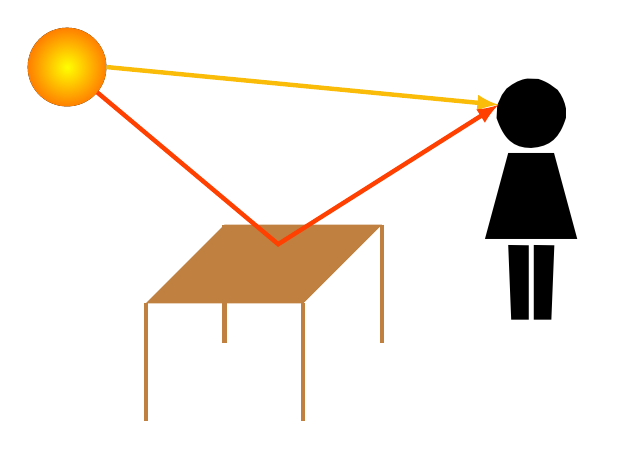
\begin{tikzpicture}
	  \fill[inner color=yellow, outer color=orange] (0,0) circle (5mm);
	  \node[anchor=north west] at (5,0) {\scalebox{12}{\Ladiesroom}};
	  \fill[brown] (2,-2) coordinate (leg1) -- ++(2,0) coordinate (leg2) --++(-1,-1) coordinate (leg3) --++(-2,0) coordinate (leg4) -- cycle;
	  \foreach \l in {leg1, leg2, leg3, leg4}{
		\draw[brown, ultra thick] (\l) --+ (0,-1.5);
	  }
	  \draw<2->[-latex,ultra thick, yellow!50!orange] (0:5mm) -- (-5:5.5);
	  \draw<3->[-latex,ultra thick, orange!50!red] (-40:5mm) -- (-40:3.5) -- (-5:5.5);
	\end{tikzpicture}
  \end{center}
\end{frame}

\begin{frame}{Processing Light Information}
  \begin{itemize}
	\item The direction the light enters the eye gives position information
	\item The wavelength of the light gives color information
  \end{itemize}
  \begin{center}
	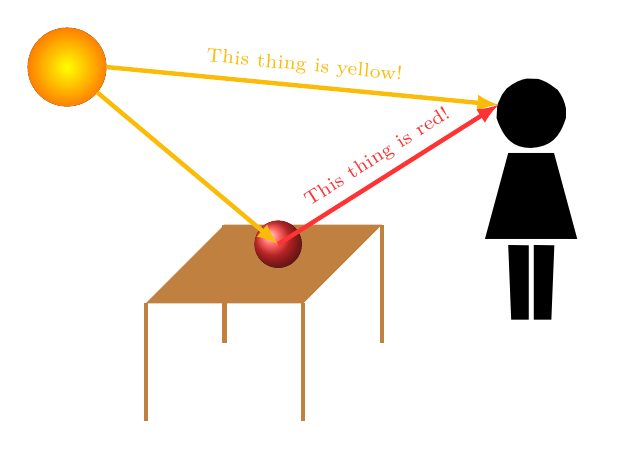
\begin{tikzpicture}
	  \fill[inner color=yellow, outer color=orange] (0,0) circle (5mm);
	  \node[anchor=north west] at (5,0) {\scalebox{12}{\Ladiesroom}};
	  \fill[brown] (2,-2) coordinate (leg1) -- ++(2,0) coordinate (leg2) --++(-1,-1) coordinate (leg3) --++(-2,0) coordinate (leg4) -- cycle;
	  \foreach \l in {leg1, leg2, leg3, leg4}{
		\draw[brown, ultra thick] (\l) --+ (0,-1.5);
	  }
	  \draw[-latex,ultra thick, yellow!50!orange] (0:5mm) -- node[midway,above,sloped, font=\scriptsize] {This thing is yellow!} (-5:5.5);
	  \fill[ball color=red!80] (-40:3.5) circle (3mm);
	  \draw[-latex,ultra thick, yellow!50!orange] (-40:5mm) -- (-40:3.5);
	  \draw[-latex,ultra thick, red!80] (-40:3.5) -- node[midway,above,sloped,font=\scriptsize] {This thing is red!} (-5:5.5);
	\end{tikzpicture}
  \end{center}
\end{frame}

%\begin{frame}{Robot Eyes}
  %\begin{itemize}
	%\item Cameras and Telescopes operate similar to our eyes
	  %\begin{itemize}
		%\item A lens focuses incoming light
		%\item Light is focused on a light sensitive region in the back
		%\item Flaws in optics cause blurry or distorted images
	  %\end{itemize}
	%\item Both record light position and color
	%\item Some cameras and telescopes can also detect incoming light's polarization
  %\end{itemize}
  %\begin{figure}[h!]
	%\centering
	%\includegraphics[width=.4\textwidth]{ch5_robot-eye.jpg}
  %\end{figure}
%\end{frame}

\begin{frame}{Tricks of Light}
  \begin{columns}
	\column{.5\textwidth}
	\begin{itemize}
	  \item<1-> A single image gives no \alert{distance} information
	  \item<2-> Light can bend, which confuses your brain
	\end{itemize}
	  \includegraphics<1>[width=\textwidth]{ch5_starfield.jpg}
	  \includegraphics<2>[width=.9\textwidth]{ch5_lightbend2.jpg}
	\column{.5\textwidth}
	\begin{figure}[h!]
	  \centering
	  \includegraphics<1>[width=\textwidth]{ch5_lightdistance.jpg}
	  \includegraphics<2>[width=\textwidth]{ch5_lightbend.jpg}
	\end{figure}
  \end{columns}
\end{frame}

\begin{frame}{But how does it work?}
  \begin{itemize}
	\item Light is, first and foremost, a wave
	  \begin{itemize}
		\item Similar to an ocean wave
		\item Affects both electric charges and magnets ``floating'' atop it
		\item Called an electromagnetic wave
	  \end{itemize}
	  \begin{center}
		%\includegraphics[width=.8\textwidth]{emwave.jpg}
		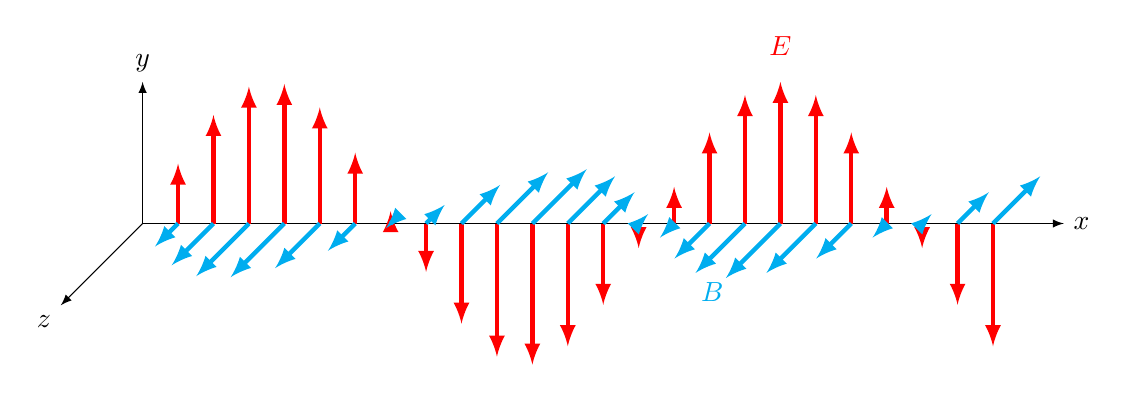
\begin{tikzpicture}[scale=.9]
		  \draw[-latex] (0,0,0) -- (13,0,0) node[right] {$x$};
		  \draw[-latex] (0,0,0) -- (0,2,0) node[above] {$y$};
		  \draw[-latex] (0,0,0) -- (0,0,3) node[below left] {$z$};
		  
		  \foreach \x in {0.5,1,...,12}{ \draw[-latex, red, ultra thick] (\x,0,0) --+(0,{2*cos(50*\x-90)},0);}
		  \foreach \x in {0.5,1,...,12}{ \draw[-latex, cyan, ultra thick] (\x,0,0) --+(0,0,{2*cos(50*\x-90)});}

		  \node[red] at (9, 2.5,0) {$E$};
		  \node[cyan] at (9, 0,2.5) {$B$};
		\end{tikzpicture}
	  \end{center}
  \end{itemize}
\end{frame}

\begin{frame}{Properties of Waves}
  \begin{center}
	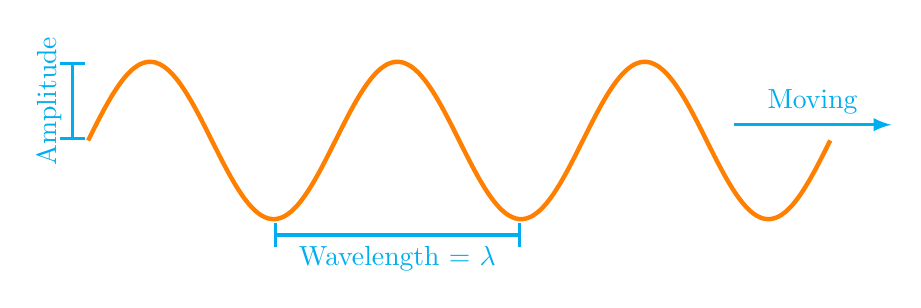
\begin{tikzpicture}
	  %\draw[help lines] (0,-1) grid (10,1);
	  \draw[scale=0.5,domain=0:6*pi, samples=100, smooth, variable=\x, ultra thick, orange] plot (\x,{2*sin(\x r)});
	  \draw[|-|, very thick, cyan] (3/4*pi,-1.2) -- node[below] {Wavelength = $\lambda$} +(pi,0);
	  \draw[very thick, cyan, -latex] (8.2,.2) -- node[above] {Moving} +(2,0);
	  \draw[|-|, very thick, cyan] (-.2,0) -- node[above,sloped] {Amplitude} +(0,1);
	\end{tikzpicture}
  \end{center}
  \begin{itemize}
	\item All light waves move at speed $c$, the speed of light:
	  \[c = \SI{3e8}{\meter\per\second}\]
	\item Amplitude corresponds to brightness
	\item Wavelength/Frequency correspond to color or portion of spectrum
  \end{itemize}
\end{frame}

\begin{frame}{The Rainbow}
  \begin{center}
	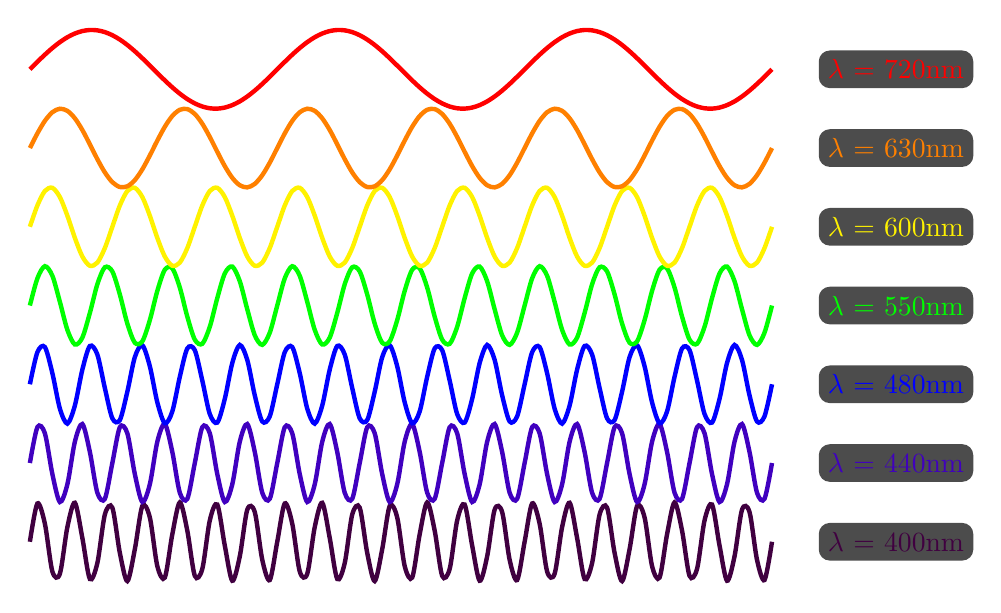
\begin{tikzpicture}
	  \foreach \f/\c/\l in {7/black!50!violet/400,6/blue!50!violet!/440,5/blue/480,4/green/550,3/yellow/600,2/orange/630,1/red/720}{
		\draw[\c,scale=0.5,domain=0:6*pi, samples=100, smooth, variable=\x, ultra thick] plot (\x,{sin(\f*\x r)-(2*\f)});
		\node[\c, fill=black!70, rounded corners] at (11,-\f) {$\lambda$ = \l \si{\nano\meter}};
	  }
	\end{tikzpicture}
  \end{center}
\end{frame}

\begin{frame}{Wavelength and Frequency}
  \begin{itemize}
	\item In a generic wave, the wavelength and frequency of a wave determine its speed
	\item Since light has a fixed speed, wavelength and frequency are related:
	  \[\lambda \times f = c\]
	  where
	  \begin{align*}
		\lambda &= \text{ wavelength} \\
		f &= \text{ frequency}
	  \end{align*}
	\item People flip back and forth in whether they use one or the other
	\item Frequencies tend to be high, so often given in \si{\tera\hertz} (\SI{1e12}{\hertz})
  \end{itemize}
\end{frame}

\begin{frame}{Understanding Check}
  A friend tells you they measured beam of light with a frequency of \SI{5e14}{\hertz}. What color is it?
  \begin{columns}
	\column{.2\textwidth}
	\begin{enumerate}
	  \item Red
	  \item \alert<2>{Yellow}
	  \item Green
	  \item Blue
	\end{enumerate}
	\column{.5\textwidth}
	\begin{center}
	  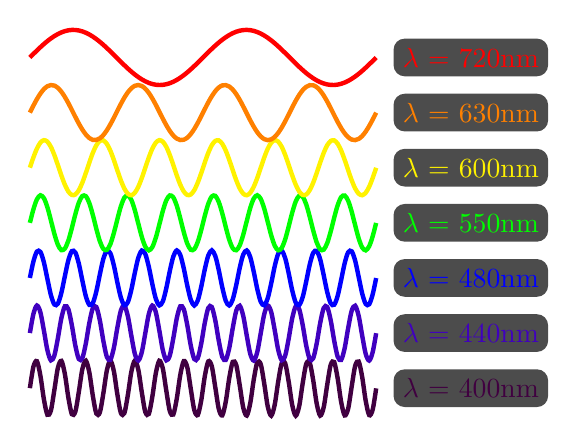
\begin{tikzpicture}[scale=.7]
		\foreach \f/\c/\l in {7/black!50!violet/400,6/blue!50!violet!/440,5/blue/480,4/green/550,3/yellow/600,2/orange/630,1/red/720}{
		  \draw[\c,scale=0.5,domain=0:4*pi, samples=100, smooth, variable=\x, ultra thick] plot (\x,{sin(\f*\x r)-(2*\f)});
		  \node[\c, fill=black!70, rounded corners] at (8,-\f) {$\lambda$ = \l \si{\nano\meter}};
		}
	  \end{tikzpicture}
	\end{center}
  \end{columns}
\end{frame}

\begin{frame}{Oh the possibilities}
  \begin{itemize}
	\item We have 4 main ways lightwaves will interact with objects
	  \begin{itemize}
		\item Emission: if the object is emitting visible light
		\item Absorption: if the object absorbs all the light (and heats up)
		\item Transmission: if the object allows light through
		\item Bouncing:
		  \begin{itemize}
			\item Reflection: if the object bounces the light perfectly
			\item Scattering: if the bouncing is messy and in all directions
		  \end{itemize}
	  \end{itemize}
  \end{itemize}
\end{frame}

\begin{frame}{Our Blue Sky}
  \begin{itemize}
	\item Molecules in the atmosphere scatter the smaller wavelength light (Blue$\rightarrow$Violet)
	\item The white light from the sun thus gets the blue bits scattered throughout the atmosphere
	\item The Earth reflects all manner of colors (so white) back up into the atmosphere as well, which lightens the shade of blue we see
	\item Why isn't the sky violet?
	  \begin{itemize}
		\item Amount of ``violet'' in sunlight is less
		\item Our eyes are less sensitive to violet
	  \end{itemize}
	\item Sunsets redder because more blue light scattered away through thicker atmosphere
  \end{itemize}
\end{frame}

\begin{frame}{Shadings of Sky}
  \begin{center}
	\begin{tikzpicture}
	  \node at (0,0) {\includegraphics[width=6cm]{ch5_bluesky.jpg}};
	  \node at (5,1) {\includegraphics[width=5cm]{ch5_spacesky.jpg}};
	  \node at (4.5,-2.2) {\includegraphics[width=6cm]{ch5_sunsetsky.jpg}};
	  \node at (-0.7,-3) {\includegraphics[width=4.5cm]{ch5_bluesky2.png}};
	\end{tikzpicture}
  \end{center}
\end{frame}

%\begin{frame}{I'm (Mostly) Blind!}
  %\begin{center}
	%\begin{tikzpicture}
	  %%Drawing the Bottom
	  %\shade[shading=rainbow] (0,0) rectangle (9,1);
	  %\draw[very thin] (0,0) rectangle (9,1);
	  %\draw (0,0) -- (9,0);
	  %\foreach \x in {0,0.5,...,9} \draw[thin] (\x,0) -- (\x,-0.1);
	  %\foreach \x/\num in {0.5/400,3/500,5.5/600,8/700}{
		  %\draw[semithick] (\x,0) -- (\x,-0.2)
			  %node[below,font=\tiny] {$\SI{\num}{\nano\meter}$};
	  %}

	  %%Drawing the Top
	  %\fill[black] (-1.5,3) -- (8.5,3) -- (9,3.5) -- (8.5,4) -- (-1.5,4) -- (-2,3.5) -- cycle;
	  %\shade[shading=rainbow] (2.1,3) coordinate (x1) rectangle +(.35,1) coordinate (p2);
	  %\foreach[count=\c] \x in {-1,0.8,...,8.1} \draw (\x,3) -- (\x,2.9) coordinate (\c);
	  %\begin{scope}[font=\tiny, below]
		%\node at (1) {$\SI{1}{\pico\meter}$};
		%\node at (2) {$\SI{1}{\nano\meter}$};
		%%\node at (3) {$\SI{1}{\micro\meter}$};
		%\node at (4) {$\SI{1}{\milli\meter}$};
		%\node at (5) {$\SI{1}{\meter}$};
		%\node at (6) {$\SI{1}{\kilo\meter}$};
	  %\end{scope}

	  %\begin{scope}[right,font=\tiny,right,color=white, text width=1cm]
	  %\node at (-1.0,3.6) {Gamma Rays};
	  %\node at (0.4,3.6) {X Rays\phantom{gamma}};
	  %\node at (1.4,3.6) {UV \phantom{gamma}};
	  %\node at (3.0,3.6) {\centering Infrared (IR)};
	  %\node at (4.6,3.6) {Microwaves \phantom{gamma}};
	  %\node at (6.6,3.6) {Radio \phantom{gamma}};
	  %\node at (7.8,3.6) {Long Radio\phantom{gamma}};
	  %\end{scope}


	  %%Connecting Bits
	  %\draw[thin] (x1) ..controls +(-90:1.5) and +(20:1).. (0,1) coordinate(z1);
	  %\draw[thin] ($(p2)-(0,1)$) coordinate (x2) ..controls +(-90:1.5) and +(170:1.2).. (9,1) coordinate(z2);
	  %%Shading the Connecting Bits
	  %\shade[shading=rainbow,opacity=0.2] (x1)..controls +(-90:1.5) and +(20:1).. (0,1) -- (9,1) ..controls +(170:1.2) and +(-90:1.5)..(x2)--cycle;
	%\end{tikzpicture}
  %\end{center}
  %\tiny{Please just pause a moment and appreciate this lovely thing that I spend forever on\ldots}
%\end{frame}

%\fullFrameImageZoomedHorizontal{ch5_deepfield.jpg}

%\begin{frame}{Everything the Light touches\ldots}
  %\begin{itemize}
	%\item Everything that emits or reflects light we can observe
	%\item The visible bits are just a tiny fraction of the huge spectrum of possibilities
	%\item Gives rise to different forms of astronomy:
	  %\begin{itemize}
		%\item Optical
		%\item Radio
		%\item Microwave
		%\item High Energy (Gamma/X Ray)
	  %\end{itemize}
  %\end{itemize}
%\end{frame}

%\begin{frame}{Some more difficult than others\ldots}
  %\begin{center}
	%\includegraphics[width=\textwidth]{ch5_Atmosphere_Opacity.pdf}
  %\end{center}
%\end{frame}

%\begin{frame}{Light is Discrete}
  %\begin{itemize}
	%\item Why do the high energy type events correspond to lower wavelengths?
	%\item An issue with the wave theory of light:
	  %\begin{itemize}
		%\item Noticed some metals would give off electrons when light was shone on them
		%\item Oddly, the intensity (amplitude) of light didn't change the number of electrons
		%\item The wavelength (or frequency) of the light DID change the number
		%\item How to explain?
	  %\end{itemize}
  %\end{itemize}
%\end{frame}

%\begin{frame}{The Photoelectric Effect}
  %\begin{center}
	%\begin{tikzpicture}
	  %\fill[pattern=north east lines, pattern color=fg] (0,0) rectangle (8,-0.5);	  
	  %\draw[very thick] (0,0) -- (8,0);
	  %\draw[decorate, decoration={snake, segment length=5mm, amplitude=2mm}, ultra thick, red] (1,0) -- +(135:3);
	  %\draw[decorate, decoration={snake, segment length=3mm, amplitude=2mm}, ultra thick, green] (3,0) -- +(135:3);
	  %\draw[dashed, ultra thick, green] (3,0) -- node[midway,sloped,below] {fast}+(60:2) node[fill,circle,inner sep=0pt, minimum size=5pt] {};
	  %\draw[decorate, decoration={snake, segment length=2mm, amplitude=2mm}, ultra thick, violet] (7,0) -- +(135:3);
	  %\draw[dashed, ultra thick, violet] (7,0) -- node[midway,sloped,below] {faster}+(60:3) node[fill,circle,inner sep=0pt, minimum size=5pt] {};
	%\end{tikzpicture}
  %\end{center}
  %\begin{itemize}
	%\item Einstein found that light transfers energy in discrete chunks, called quanta
	%\item The energy in each quanta is related to the wavelength
	  %\begin{itemize}
		%\item Smaller wavelengths (higher frequency) = higher energy
	  %\end{itemize}
  %\end{itemize}
  %\begin{alertblock}{Light: Because life is complicated}
	%Light behaves both like a wave \emph{and} like a particle!
  %\end{alertblock}
%\end{frame}

%\begin{frame}{Back to the Spectrum}
  %\begin{center}
	%\begin{tikzpicture}
	  %%Drawing the Bottom
	  %\shade[shading=rainbow] (0,0) rectangle (9,1);
	  %\draw[very thin] (0,0) rectangle (9,1);
	  %\draw (0,0) -- (9,0);
	  %\foreach \x in {0,0.5,...,9} \draw[thin] (\x,0) -- (\x,-0.1);
	  %\foreach \x/\num in {0.5/400,3/500,5.5/600,8/700}{
		  %\draw[semithick] (\x,0) -- (\x,-0.2)
			  %node[below,font=\tiny] {$\SI{\num}{\nano\meter}$};
	  %}

	  %%Drawing the Top
	  %\fill[black] (-1.5,3) -- (8.5,3) -- (9,3.5) -- (8.5,4) -- (-1.5,4) -- (-2,3.5) -- cycle;
	  %\shade[shading=rainbow] (2.1,3) coordinate (x1) rectangle +(.35,1) coordinate (p2);
	  %\foreach[count=\c] \x in {-1,0.8,...,8.1} \draw (\x,3) -- (\x,2.9) coordinate (\c);
	  %\begin{scope}[font=\tiny, below]
		%\node at (1) {$\SI{1}{\pico\meter}$};
		%\node at (2) {$\SI{1}{\nano\meter}$};
		%%\node at (3) {$\SI{1}{\micro\meter}$};
		%\node at (4) {$\SI{1}{\milli\meter}$};
		%\node at (5) {$\SI{1}{\meter}$};
		%\node at (6) {$\SI{1}{\kilo\meter}$};
	  %\end{scope}

	  %\begin{scope}[right,font=\tiny,right,color=white, text width=1cm]
	  %\node at (-1.0,3.6) {Gamma Rays};
	  %\node at (0.4,3.6) {X Rays\phantom{gamma}};
	  %\node at (1.4,3.6) {UV \phantom{gamma}};
	  %\node at (3.0,3.6) {\centering Infrared (IR)};
	  %\node at (4.6,3.6) {Microwaves \phantom{gamma}};
	  %\node at (6.6,3.6) {Radio \phantom{gamma}};
	  %\node at (7.8,3.6) {Long Radio\phantom{gamma}};
	  %\end{scope}

	  %\node[violet!50,anchor=west] at (-1,4.5) {Higher Energies};
	  %\node[red!50,anchor=west] at (5.5,4.5) {Lower Energies};

	  %%Connecting Bits
	  %\draw[thin] (x1) ..controls +(-90:1.5) and +(20:1).. (0,1) coordinate(z1);
	  %\draw[thin] ($(p2)-(0,1)$) coordinate (x2) ..controls +(-90:1.5) and +(170:1.2).. (9,1) coordinate(z2);
	  %%Shading the Connecting Bits
	  %\shade[shading=rainbow,opacity=0.2] (x1)..controls +(-90:1.5) and +(20:1).. (0,1) -- (9,1) ..controls +(170:1.2) and +(-90:1.5)..(x2)--cycle;
	%\end{tikzpicture}
  %\end{center}
%\end{frame}

%\begin{frame}{How to make some light\ldots}
  %\begin{itemize}
	%\item The general term \underline{electromagnetic radiation} describes all the frequencies, not just the visible ones we generally call ``light''
	%\item How do we produce EM-radiation?
	  %\begin{itemize}[<+->]
		%\item Take something hot\ldots
		%\item \ldots or warm \ldots
		%\item \ldots or not 100\%, absolutely cold
	  %\end{itemize}
	%\item What wavelengths are emitted depend on the objects temperature
	  %\begin{itemize}[<+->]
		%\item Hot object produce more radiation in general
		%\item Hot objects produce more radiation at shorter wavelengths
	  %\end{itemize}
  %\end{itemize}
%\end{frame}

%\begin{frame}{A shining example \footnotesize(ba-dump tssh)}
  %\begin{columns}
	%\column{.5\textwidth}
	%\begin{itemize}
	  %\item Star color depends on the star's temperature!
	  %\item The brightness we see also depends on the star's size and distance from us (more on that later!)
	%\end{itemize}
	%\column{.5\textwidth}
	%\begin{center}
	  %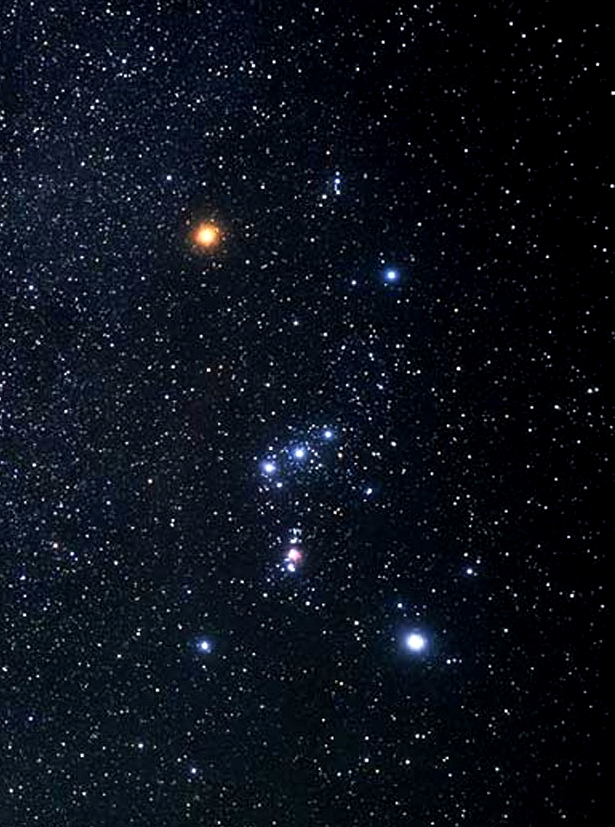
\includegraphics[width=.7\textwidth]{ch5_orion.jpg}
	%\end{center}
  %\end{columns}
%\end{frame}


\end{document}
